\chapter{CMB and matter power spectra}\label{ch:cmb-spectra}
\chapterstatus{written}{2026-11-14}

This chapter turns the source functions and transfer functions of \cref{ch:linear-perturbations} into observables:
the angular power spectra of the CMB temperature and polarization by line-of-sight integration, their lensing, the
contributions of tensor and isocurvature modes, the linear matter power spectrum, and real-space two-point functions.
It also describes the Einstein--Boltzmann solver as a program and a library.

\begin{modulebox}{Cosmology/Spectra and Cosmology/EinsteinBoltzmannSolver}
\file{Cosmology/Spectra}: \file{PowerSpectrum.h/.cpp} (class \cls{PowerSpectrum}: line of sight, $C_\ell$, $P(k)$),
\file{Lensing.cpp}, \file{HypersphericalBessel.cpp}, \file{TwoPoint.h/.cpp}, \file{PowerSpectrumTwoPoint.cpp},
\file{EisensteinHu.h}, \file{Halofit.cpp}, \file{PowerSpectrumReACT.cpp}, \file{NONLINEAR.md}.\par
\file{Cosmology/Perturbations}: \file{Tensors.h/.cpp}, \file{Isocurvature.h}.\par
\file{Cosmology/EinsteinBoltzmannSolver}: \file{EinsteinBoltzmannSolver.h/.cpp} (class
\cls{EinsteinBoltzmannSolver}), \file{Main.cpp} (the program \code{cmb}), \file{ParameterFile.h/.cpp},
\file{params/*.ini}, \file{README.md}, \file{OPTIONS.md}, \file{DEVELOPING.md}, \file{report/paper.pdf}.
\end{modulebox}

\section{Primordial spectra}

Every mode of \cref{ch:linear-perturbations} is normalised to $\mathcal R=1$, so every observable is a primordial
amplitude times a transfer function. The primordial curvature spectrum is
\begin{equation}
\mathcal P_\mathcal R(k)=A_s\left(\frac{k}{k_{\rm pivot}}\right)^{n_s-1+\frac12\alpha_s\ln(k/k_{\rm pivot})}
\end{equation}
(\param{A_s}, \param{n_s}, \param{alpha_s}, \param{k_pivot} $=0.05\Mpc^{-1}$), and the tensor spectrum
$\mathcal P_t=rA_s(k/k_{\rm pivot})^{n_t}$ with $n_t=-\frac r8\left(2-\frac r8-n_s\right)$ by default (the slow-roll
consistency relation, CLASS's \code{n_t = scc}; \param{n_t_consistency}, \param{n_t}).

\section{The line-of-sight integral}\label{sec:cmb-los}

Solving the photon hierarchy to $\ell\sim2500$ would require thousands of equations per mode. Seljak and Zaldarriaga
\cite{Seljak1996} noted that \cref{eq:pert-boltzmann} can be integrated formally along the photon path: with the
integrating factor $e^{ik\mu\eta-\tau}$, the Rayleigh expansion of the plane wave in spherical Bessel functions, and
integration by parts of the $\mu$-dependent terms,
\begin{equation}
\Theta_\ell(k)=\int_{-\infty}^0S_T(k,x)\,j_\ell[k(\eta_0-\eta)]\,\dd x,\qquad
\Theta^E_\ell(k)=\sqrt{\frac{(\ell+2)!}{(\ell-2)!}}\int_{-\infty}^0S_E(k,x)\,j_\ell[k(\eta_0-\eta)]\,\dd x,
\label{eq:cmb-los}
\end{equation}
with the sources of \cref{eq:pert-ST,eq:pert-SE}. This separates the physics (the sources, smooth in $k$ and needing
only low multipoles) from the geometry (the projection onto multipole $\ell$ at distance $\eta_0-\eta$). The angular
spectra are
\begin{equation}
C_\ell^{XY}=4\pi\int_0^\infty\frac{\dd k}{k}\,\mathcal P_\mathcal R(k)\,\Theta^X_\ell(k)\,\Theta^Y_\ell(k),\qquad
X,Y\in\{T,E\},
\label{eq:cmb-cl}
\end{equation}
reported as $D_\ell=\ell(\ell+1)C_\ell/2\pi$ in $\mu$K$^2$ (multiplied by $(10^6T_{\rm CMB})^2$). On large scales only
the Sachs--Wolfe term contributes and a scale-invariant spectrum gives the plateau $D_\ell\simeq A_sT_{\rm CMB}^2/25$;
the acoustic peaks sit at $\ell_n\approx n\ell_A-\phi_n$ with $\ell_A=\pi\chi_*/r_{s*}$, and diffusion damping
suppresses the power above $\ell_D=k_D\chi_*\approx2000$.

\begin{implementation}[Implementation: line of sight and $k$ integration]
\begin{itemize}
\item $j_\ell(z)$ is tabulated for all needed $\ell$ on a uniform grid with \param{bessel_points_per_2pi} $=32$
      points per $2\pi$ (and $j_\ell(z)/z^2$ for the $E$ source), for $O(1)$ lookups.
\item The $x$-integral (trapezoidal) starts at \param{x_start_los} $=-8.5$, where $e^{-\tau}$ makes the sources
      negligible; spacing \param{dx_recomb} $=0.003$ in $[\code{x_recomb_min},\code{x_recomb_max}]=[-7.6,-6.2]$ to
      resolve $\gt$, elsewhere uniform in $\eta$ with \param{n_eta_per_oscillation} $=5$ points per Bessel oscillation at
      $k_{\max}$.
\item The $k$-integral uses \param{n_k_per_oscillation} $=4$ points per period $2\pi/\eta_0$ of the transfer
      functions and $\Delta\ln k\le$ \param{dlnk_max} $=0.02$ at small $k$, over $[\code{los_k_min},\code{los_k_max}]$
      (default: the perturbation range). Do not set $k_{\max}$ much below $0.3\Mpc^{-1}$ for the $C_\ell$: $k_{\max}
      r_*>\ell$ is only a minimum.
\item $C_\ell$ is computed at a list of multipoles (\param{ells}, or every \param{ell_step} $=25$ above
      $\ell=100$, up to \param{ell_max}) and splined in $\ell$.
\item Doubling the line-of-sight and $k$ sampling changes the spectra by $<5\times10^{-5}$.
\end{itemize}
\end{implementation}

\subsection{Curved universes}

In a curved universe the projection uses the hyperspherical Bessel functions $\Phi^\nu_\ell(\chi)$ ($\chi$ in units of
the curvature radius), which solve
\begin{equation}
\Phi''+2\cot_K\chi\,\Phi'+\left[\nu^2-\mathrm{sgn}K-\frac{\ell(\ell+1)}{\sin_K^2\chi}\right]\Phi=0,
\end{equation}
with $\Phi^\nu_0=\sin(\nu\chi)/(\nu\sin_K\chi)$ and the recurrence
$\sqrt{\nu^2-\mathrm{sgn}K(\ell+1)^2}\,\Phi_{\ell+1}=(2\ell+1)\cot_K\chi\,\Phi_\ell-\sqrt{\nu^2-\mathrm{sgn}K\ell^2}\,
\Phi_{\ell-1}$; they reduce to $j_\ell(\nu\chi)$ for $\nu\to\infty$. The integration by parts of \cref{eq:pert-ST} is
not available, so the three parts of the source are projected separately \cite{LesgourguesTram2014}:
\begin{align}
\Theta_\ell(k)&=\int\dd x\left[S_{T0}\Phi_\ell+S_{T1}\frac{\sqrt{|K|}}{k}\Phi_\ell'
+S_{T2}\frac{3(|K|/k^2)\Phi_\ell''+\Phi_\ell}{2s_2}\right],\\
\Theta^E_\ell(k)&=\sqrt{\frac{(\ell+2)!}{(\ell-2)!}}\int\dd x\,\frac{3\gt\,\Pi}{4}\,\frac{\Phi_\ell}{s_2(kr)^2},
\end{align}
and in a closed universe the $k$-integral becomes a sum over integer $\nu$.

\begin{implementation}[Implementation: hyperspherical Bessel functions]
$\Phi^\nu_\ell$ is computed by upward recurrence below the turning point $\ell(\ell+1)=(\nu^2-\mathrm{sgn}K)\sin_K^2\chi$,
where it oscillates, and by Miller's downward recurrence above it \cite{Kosowsky1998,Tram2017} (starting exactly at
$\ell=\nu-1$ in a closed universe). For $\nu\ge$ \param{flat_approximation_nu} $=4000$ CLASS's flat approximation
replaces $\Phi^\nu_\ell$ by a rescaled $j_\ell$ with an amplitude correction ($\lesssim6\times10^{-4}$ in $C_\ell$ at
$\Om_k=\pm0.05$). The closed-universe sum uses a uniform integer stride in $\nu$ (rounding a uniform $k$ grid gave
irregular strides and 4\% errors). Modes with small $q$ use a proportionally coarser $x$-grid away from
recombination, never coarser than \param{dx_max_subsampled} $=0.01$. Tests: agreement with $j_\ell$ when flat to
$2\times10^{-12}$, the radial equation, the closed-form Gegenbauer functions to $10^{-13}$, and the $1/\nu^2$ approach
to $j_\ell$. \param{use_radial_functions} forces this path in a flat universe as a test (agreement with the
integrated-by-parts result to $5\times10^{-5}$).
\end{implementation}

\begin{figure}[htbp]
\centering
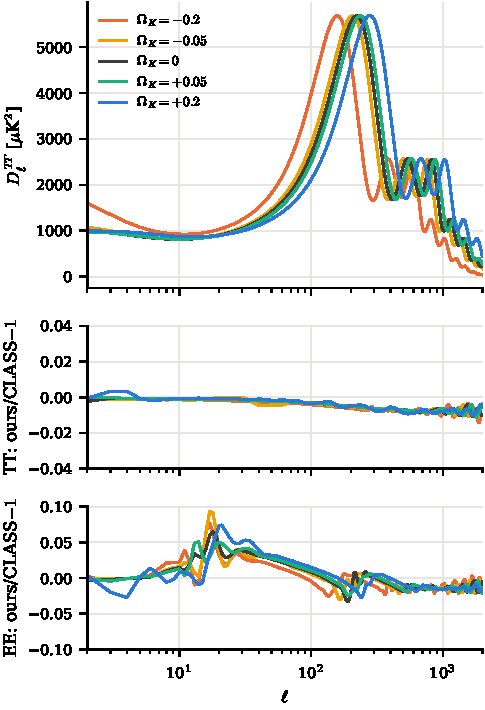
\includegraphics[width=0.6\textwidth]{curvature_spectra}
\caption{\emph{Top:} TT spectra for $\Omega_K=-0.2$, $-0.05$, 0, 0.05 and 0.2 at fixed matter and baryon density. \emph{Middle and bottom:} TT
and EE relative to CLASS with the same physics (unlensed). From the solver report.}
\label{fig:cmb-curvature}
\end{figure}


\section{The matter power spectrum}\label{sec:cmb-pk}

The matter power spectrum uses the comoving-gauge (synchronous-gauge, as CLASS) density contrast of the clustering
species,
\begin{equation}
\Delta_m(k,x)=\frac{\sum_i\rho_i\left[\delta_i-3(1+w_i)\Hp v_i/(ck)\right]}{\sum_i\rho_i},\qquad
P(k,x)=|\Delta_m(k,x)|^2\,\frac{2\pi^2}{k^3}\mathcal P_\mathcal R(k),
\end{equation}
summed over CDM, baryons and massive neutrinos for $P_m$ (and the ultralight axion when $m\ge10^{-25}$\,eV), and over
CDM and baryons for $P_{cb}$, the spectrum relevant for galaxy clustering in the presence of neutrinos. Inside the
horizon this is the Newtonian density contrast; it is consistent with the Poisson equation
$\Delta_m=\frac23\frac{c^2k^2}{\Hp^2}\frac{\Phi}{\Om_m(x)}$ up to radiation terms of order $10^{-3}$ on the largest
scales. $\sigma_R$ and $\sigma_8$ follow by integrating with the top-hat window; beyond the computed $k$-range $\Delta_m$
is extrapolated with the shape of the Eisenstein--Hu no-wiggle transfer function \cite{EisensteinHu1998} anchored at
$k_{\max}$ (\code{get_matter_power_spectrum_extrapolated}).

\paragraph*{Massive neutrinos} suppress $P_m$ below the free-streaming scale by $\approx-8f_\nu$ asymptotically
($f_\nu=\Om_\nu/\Om_m$): $2f_\nu$ from the non-clustering fraction and the rest from the slower growth
$\delta_{cb}\propto a^{1-3f_\nu/5}$ \cite{HuEisensteinTegmark1998,LesgourguesPastor2006}. The code reproduces CLASS's
suppression (16.1\% against 16.2\% at $k=0.5\hMpc$ for $m_\nu=0.3$\,eV; \cref{fig:cmb-neutrinos}).

\paragraph*{Nonlinear power.} \param{nonlinear} selects a nonlinear prescription (\code{halofit},
\code{halofit_bird}, \code{hmcode2016}, \code{hmcode2020}, \code{react}, \code{ee2}, \code{jbd_boost},
\code{axionhmcode}), added as a column of the output and used for the nonlinear lensing potential (the Weyl
potential of the Limber part is scaled by $\sqrt{P_{\rm NL}/P_{\rm L}}$). The methods are described in
\cref{ch:halo-model,ch:fitting-emulators}.

\begin{figure}[htbp]
\centering
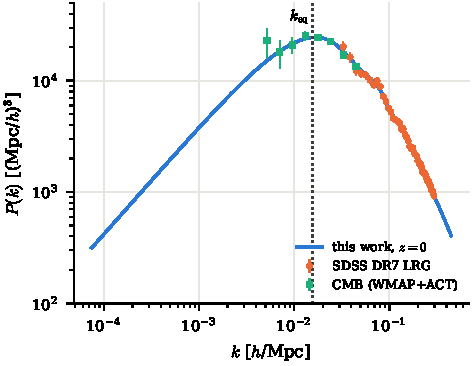
\includegraphics[width=0.6\textwidth]{m4_Pk}
\caption{The linear matter power spectrum today compared with the SDSS DR7 luminous red galaxy power spectrum \cite{Reid2010} and an estimate
from WMAP and ACT CMB data; the dotted line marks $k_{\rm eq}$. From the solver report.}
\label{fig:cmb-pk}
\end{figure}


\section{CMB lensing}\label{sec:cmb-lensing}

The CMB photons are deflected by the intervening structure: the observed temperature in direction $\hat{\bm n}$ is the
unlensed one at $\hat{\bm n}+\nabla\phi$, with the lensing potential
\begin{equation}
\phi(\hat{\bm n})=-\int_0^{\chi_*}\dd\chi\,\frac{\sin_K(\chi_*-\chi)}{\sin_K(\chi_*)\sin_K(\chi)}
\left(\Psi-\Phi\right)(\chi\hat{\bm n},\eta_0-\chi),
\end{equation}
the projection of the Weyl potential that bends light, with the last-scattering surface treated as one source plane
at the peak of $\gt$. $C_\ell^{\phi\phi}$ is computed with the line-of-sight machinery below \param{lensing_limber_ell}
$=30$ and with the Limber approximation above,
\begin{equation}
C_\ell^{\phi\phi}\simeq\int\dd\chi\,\frac{W^2(\chi)}{\sin_K^2\chi}\,
P_{\Psi-\Phi}\!\left(\frac{\ell+\frac12}{\sin_K\chi},\chi\right),
\end{equation}
with the Weyl potential extrapolated beyond $k_{\max}$ as $\ln k/k^2$; the two agree to $0.2\%$ for $40\le\ell\le200$.
The lensed spectra use the full-sky correlation-function method of Challinor and Lewis \cite{Challinor2005}, as in
CLASS: the lensed correlation functions are the unlensed ones with the deflection averaged, e.g.
\begin{equation}
\tilde\xi(\beta)=\sum_\ell\frac{2\ell+1}{4\pi}C_\ell\,e^{-\ell(\ell+1)\sigma^2(\beta)/2}d^\ell_{00}(\beta)+\ldots,
\end{equation}
where $\sigma^2(\beta)$ is the variance of the relative deflection of two points at separation $\beta$ and the dots
are terms of first and second order in the anisotropic part $C_{{\rm gl},2}(\beta)$. Polarization uses $\xi_\pm$ and
$\xi_\times$ with the Wigner functions $d^\ell_{22}$, $d^\ell_{2-2}$, $d^\ell_{20}$ (three-term recurrences). The lensed
spectra follow by Gauss--Legendre integration over $\cos\beta$. Lensing couples multipoles over
$\Delta\ell\sim$ hundreds, so the unlensed spectra are computed to $\ell_{\max}+$ \param{lensing_delta_ell}
(default $\max(500,\ell_{\max}/3)$). Lensing smooths the peaks (+3.4\% at the trough at $\ell=1000$), transfers power
to the damping tail and converts $E$ into $B$ modes ($D_\ell^{BB}$ peaks at $\approx0.09\muK$ near $\ell\approx900$).
Enable it with \param{lensing} \code{= true}.

\begin{figure}[htbp]
\centering
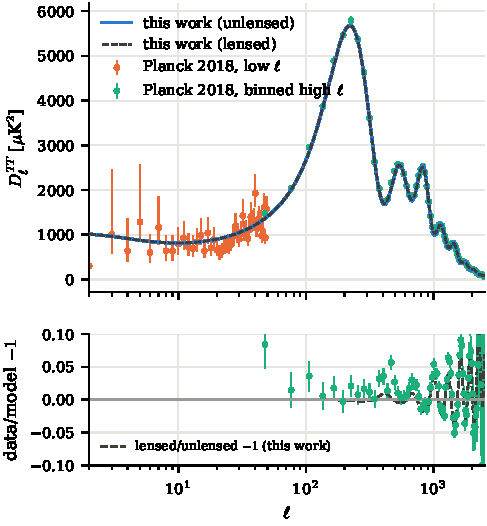
\includegraphics[width=0.49\textwidth]{m4_TT_planck}\hfill
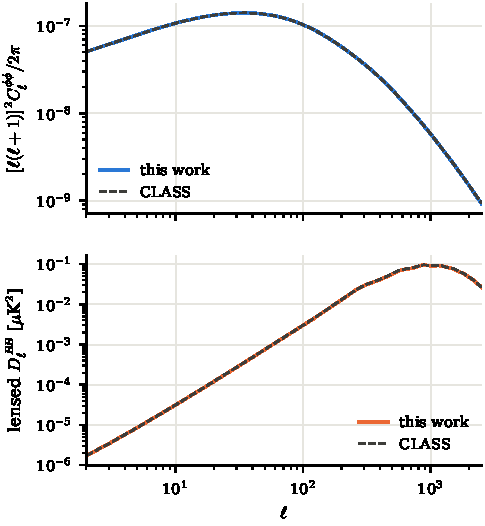
\includegraphics[width=0.49\textwidth]{m4_lensing}
\caption{\emph{Left:} unlensed and lensed TT spectra of the fiducial model compared with the Planck 2018 data
\cite{Planck2018spectra}, and the residuals. \emph{Right:} the lensing potential and the lensing $B$ modes against
CLASS (dashed). From the solver report, computed with the Peebles recombination model.}
\label{fig:cmb-tt}
\end{figure}

\begin{figure}[htbp]
\centering
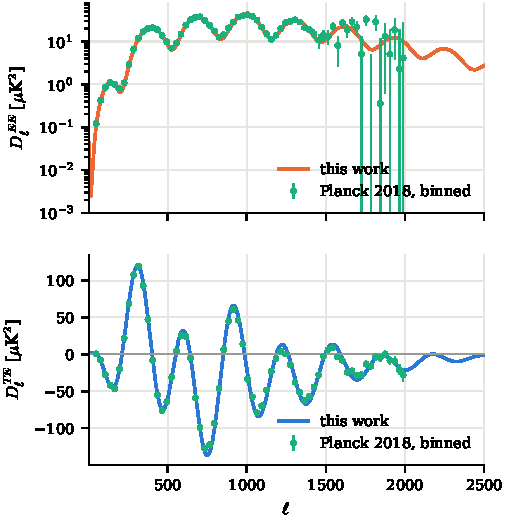
\includegraphics[width=0.49\textwidth]{m4_EE_TE}\hfill
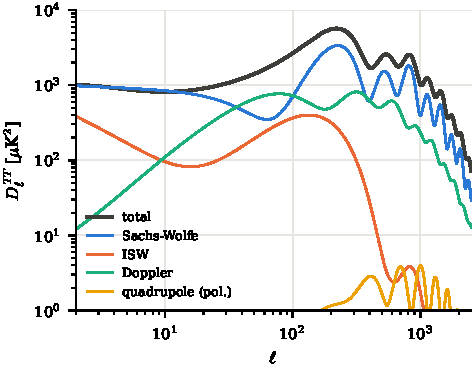
\includegraphics[width=0.49\textwidth]{m4_TT_components}
\caption{\emph{Left:} $E$-mode polarisation and the temperature--polarisation cross spectrum compared with binned Planck 2018 data.
\emph{Right:} the contributions to TT from the four terms of the temperature source function (Sachs--Wolfe, ISW, Doppler, polarisation),
each computed alone; they add in amplitude, not in power. From the solver report (Peebles recombination).}
\label{fig:cmb-ee-te}
\end{figure}


\section{Tensor modes}\label{sec:cmb-tensors}

With \param{r} $>0$ the solver adds primordial gravitational waves. The tensor perturbation $h$ obeys
\begin{equation}
\ddot h+(2+\alpha_M)\Hp\dot h+c^2k^2h=\frac{16\pi Ga^2}{M_*^2}\,\Pi_T
\end{equation}
(dots: conformal time), sourced by the tensor anisotropic stress $\Pi_T$ of photons and neutrinos, with the friction
$\alpha_M$ and the effective Planck mass $M_*^2$ of the theory of gravity (Horndeski $\alpha_M$, Brans--Dicke $\phi$,
$f(R)$ $1+f_R$; GR otherwise). The photon temperature and polarization and the neutrino tensor hierarchies are those
of CLASS (flat), with tight coupling; massive neutrinos are evolved with the massless hierarchy and weighted by
$3p_{\rm ncdm}$ in the stress (CLASS's \code{tensor_method = massless}). Tensor TT, EE, TE are added to the scalar
spectra, BB is the tensor one, and all are lensed together. Settings: \param{tensor_k_max}, \param{tensor_dk_max},
\param{tensor_k_fine}, \param{tensor_n_k_per_oscillation}, \param{tensor_lmax}, \param{tensor_lmax_nu},
\param{tensor_neutrinos}, \param{tensor_ell_max} $=600$. Flat universes only; about 10\,s on two cores.

\begin{validation}[Validation: tensors]
\begin{itemize}
\item Against CLASS ($r=0.1$): unlensed tensor TT, EE, BB to 0.1--0.5\% for $\ell\le300$; lensed total BB to
      $0.1\%$ for $\ell=50$--300.
\item The damping of the amplitude by neutrino free streaming: $\times0.8026$ (Weinberg's value \cite{Weinberg2004}).
\item Matter era without stress: $h=3j_1(k\eta)/(k\eta)$ to $0.2\%$; Horndeski $c_M=0.5$: $h\propto1/(aM_*)$ to $10^{-3}$.
\end{itemize}
\end{validation}

\section{Isocurvature modes}\label{sec:cmb-isocurvature}

The CDM, baryon, neutrino density and neutrino velocity isocurvature modes (\param{f_cdi}, \param{f_bi},
\param{f_nid}, \param{f_niv}, with tilts \code{n_*} and correlations \code{c_ad_*} with the adiabatic mode, in
CLASS's conventions) have $P_{II}=f^2A_s(k/k_{\rm pivot})^{n_I-1}$ and $P_{\mathcal RI}=c\sqrt{P_{\mathcal R\mathcal R}
P_{II}}$; the isocurvature modes are uncorrelated with each other and $\sum c^2<1$. Their superhorizon initial
conditions are CLASS's series \cite{BucherMoodleyTurok2000}. The correlation matrix is Cholesky-factored into
independent components, each one perturbation solve with a mixture of adiabatic and isocurvature initial conditions
and one line-of-sight pass, and the $C_\ell$, $C_\ell^{\phi\phi}$ and $P(k)$ are summed over the components. For
\code{model = axion}, \param{f_axi} is the density isocurvature of the axion, or \param{ax_log10_Hinf} sets it from
the field fluctuation $\delta\phi=H_{\rm inf}/2\pi$: $f_{\rm axi}^2A_s=H_{\rm inf}^2/(\pi^2\phi_i^2)$,
$n_{\rm axi}=1-r/8$. Isocurvature modes require GR and the standard species. Against CLASS the pure CDI and NID modes
agree to $5\times10^{-4}$ in TT and EE for $10\le\ell\le600$.

\section{Two-point functions}\label{sec:cmb-twopoint}

\paragraph*{CMB correlation functions.} For a statistically isotropic sky
$C(\theta)=\sum_\ell\frac{2\ell+1}{4\pi}C_\ell B_\ell^2P_\ell(\cos\theta)$, with an optional Gaussian beam
$B_\ell=e^{-\ell(\ell+1)\sigma_b^2/2}$ (\param{cmb_correlation_beam_fwhm}); for polarization
$\xi_\pm=\sum_\ell\frac{2\ell+1}{4\pi}(C_\ell^{EE}\pm C_\ell^{BB})d^\ell_{2,\pm2}$ and
$\xi_X=\sum_\ell\frac{2\ell+1}{4\pi}C_\ell^{TE}d^\ell_{20}$ \cite{Challinor2005}.

\paragraph*{Matter correlation function.} $\xi(r)=\frac{1}{2\pi^2r}\int_0^\infty\dd k\,kP(k)\sin(kr)$ is computed with
Filon's method \cite{Filon1929} ($kP(k)$ linear between tabulated points, the product with $\sin kr$ integrated
analytically), so the grid only needs to resolve $P(k)$ and its BAO wiggles. The BAO peak appears at
$r\approx100\Mpch$; $\sigma_8$ agrees with CLASS to $4\times10^{-5}$.

\paragraph*{Projected density.} For a tracer with redshift distribution $n(z)$ (Gaussian, \param{angular_z},
\param{angular_sigma_z}) and linear bias \param{angular_bias},
\begin{equation}
C_\ell=4\pi\int\frac{\dd k}{k}\mathcal P_\mathcal R(k)\Delta_\ell(k)^2,\qquad
\Delta_\ell(k)=\int\dd\chi\,W(\chi)\,b\,\Delta_m(k,\chi)\,j_\ell(k\chi),
\end{equation}
exactly below $\ell=200$ and with the Limber approximation \cite{Limber1953,LoVerde2008}
$C_\ell=\int\dd\chi\,W^2b^2P((\ell+\frac12)/\chi,\chi)/\chi^2$ above; $w(\theta)$ follows from the Legendre sum. Only
the density term is included (no RSD, magnification or relativistic terms). These agree with CLASS's number-count
spectra to $2\times10^{-3}$.

\begin{figure}[htbp]
\centering
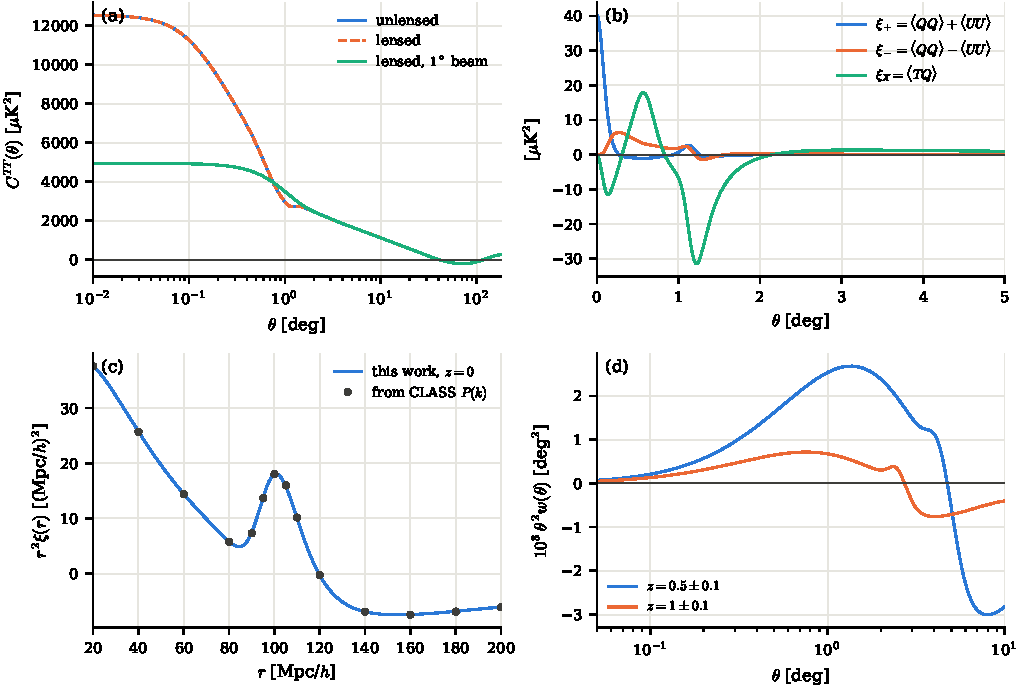
\includegraphics[width=0.85\textwidth]{twopoint}
\caption{Two-point functions of the fiducial model: (a) the CMB temperature correlation function, unlensed, lensed and with a $1^\circ$ beam;
(b) the polarisation correlation functions; (c) the matter correlation function today with the BAO peak, against the transform of CLASS's
$P(k)$; (d) the angular correlation function of matter projected over Gaussian redshift distributions ($\sigma_z=0.1$, $b=1$). From the
solver report.}
\label{fig:cmb-twopoint}
\end{figure}


\section{The solver as a program and a library}\label{sec:cmb-solver}

\paragraph*{Program.} \code{make} in \file{Cosmology/EinsteinBoltzmannSolver} builds \code{./cmb}:
\begin{paramfile}[Running the solver]
./cmb                                              # the fiducial model
./cmb params/planck2018.ini                        # parameters from a file
./cmb m_nu=0.06 lensing=true output_dir=data/test  # command-line values override the file
./cmb --write-defaults my.ini                      # every parameter with its default and description
\end{paramfile}
Every cosmological, precision and output parameter can be set in a file (\code{name = value}, \code{\#} comments) or
on the command line; unknown names are errors. \param{preset} \code{= planck2018} or \code{planck2018_baseline} loads a
parameter set; \param{precision} \code{= fast} sets precision parameters tuned for CMB likelihoods (lensed TT, EE, TE to
$\ell=2500$ in 13--16\,s instead of $\sim70$\,s, $\Delta\chi^2\approx0.2$ for Planck-like noise). The outputs are
\file{background.txt}, \file{recombination.txt}, \file{perturbations_k<k>.txt}, \file{cells.txt} ($D_\ell^{TT,EE,TE}$
in $\mu$K$^2$), \file{cells_lensed.txt}, \file{matter_power.txt} ($k$ in $\hMpc$, $P_m$, $P_{cb}$, $P_{\rm NL}$,
$P_{\rm axion}$), \file{transfer.txt}, and optionally the correlation functions and angular spectra; each run also
writes \file{params_used.ini}.

\paragraph*{Library.}
\begin{cppcode}[The solver from code]
#include <FML/Cosmology/EinsteinBoltzmannSolver/EinsteinBoltzmannSolver.h>
using namespace FML::COSMOLOGY;

auto ebs = EinsteinBoltzmannSolver::from_file("params/planck2018.ini", {"lensing=true"});
ebs.solve();                                      // or solve(Stage::Perturbations)
const auto & ps = ebs.power_spectrum();
double sigma8 = ps.get_sigma8();
double DTT    = ps.get_Dell_TT_lensed(1000);      // muK^2
double Pk     = ps.get_matter_power_spectrum(0.0, 0.1 / FML::UTILS::SI::Mpc);  // x = 0, k in 1/m
ebs.output();                                     // the files enabled in the settings
\end{cppcode}
The solver is also used by SimulationCode for its initial conditions (\code{ic_type_of_input = internal},
\cref{ch:growth-transfer}) and as the theory code of CosmologyFitting (\cref{ch:sampling-fitting}).

\begin{figure}[htbp]
\centering
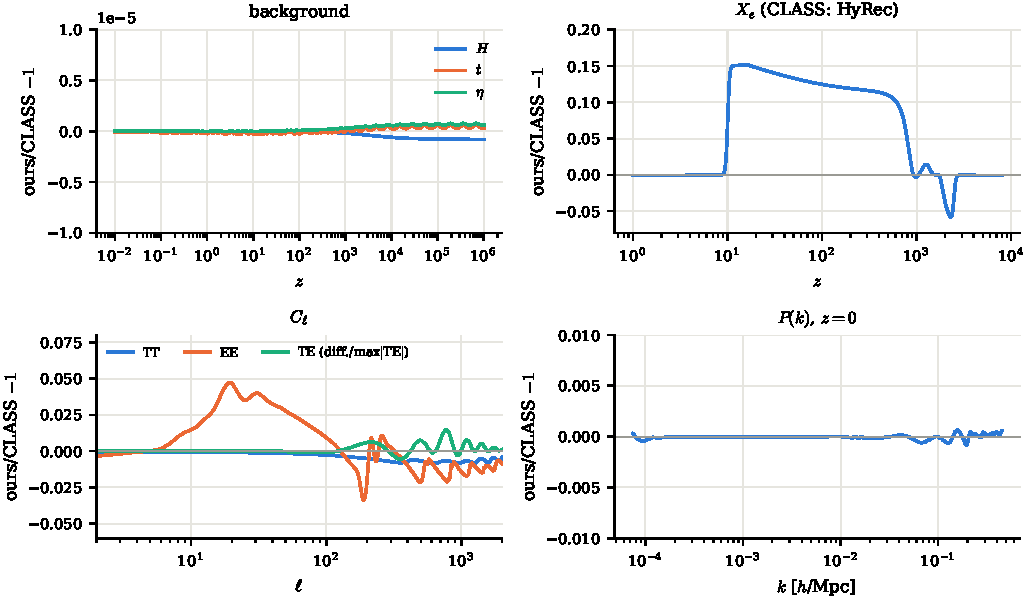
\includegraphics[width=\textwidth]{validation_class}
\caption{Comparison of the solver with CLASS run with the same physics: background, recombination, the unlensed and
lensed CMB spectra and $P(k)$. From the solver report.}
\label{fig:cmb-validation}
\end{figure}

\begin{figure}[htbp]
\centering
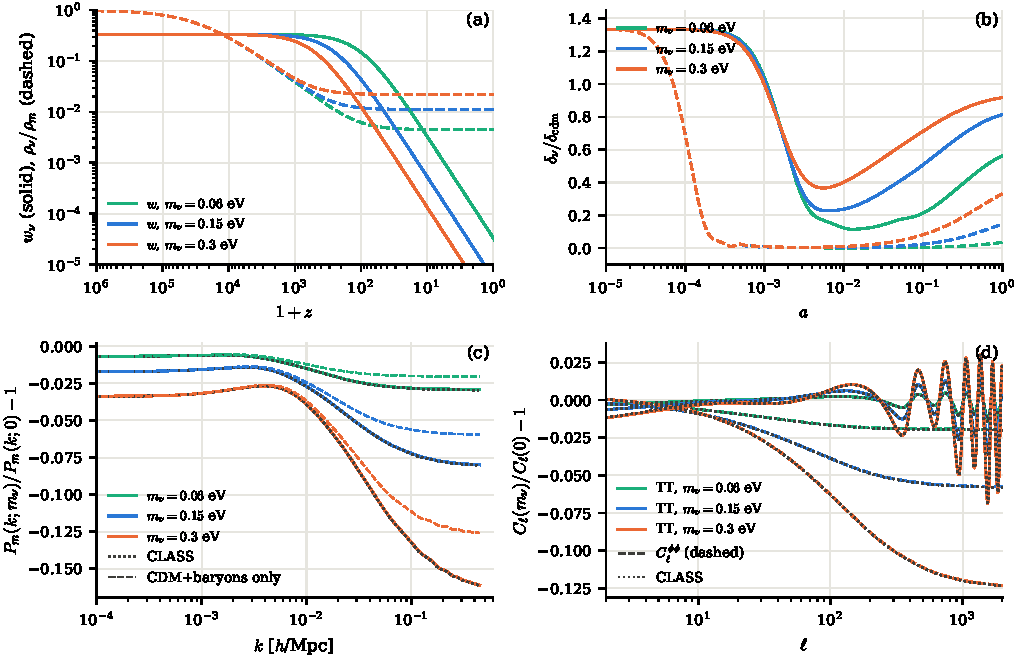
\includegraphics[width=\textwidth]{neutrinos}
\caption{Massive neutrinos with $m_\nu=0.06$, $0.15$ and $0.3$\,eV at fixed $h$, $\omega_b$, $\omega_{\rm cdm}$: the
equation of state, $\delta_\nu/\delta_{\rm cdm}$, the change of $P_m$ and $P_{cb}$, and of TT and
$C_\ell^{\phi\phi}$, with CLASS (dotted). From the solver report.}
\label{fig:cmb-neutrinos}
\end{figure}

\begin{validation}[Validation: the solver against CLASS (same physics, RECFAST)]
\begin{center}\small
\begin{tabular}{@{}ll@{}}
\toprule
Quantity & Agreement \\
\midrule
Background ($H$, $t$, $\eta$) & $10^{-7}$ \\
$X_e$ ($0\le z\le8000$) & $3\times10^{-4}$ \\
$z_*$, $r_s(z_*)$ & $10^{-6}$ \\
TT (rms, $30\le\ell\le1000$; $1000<\ell\le2000$) & $5\times10^{-4}$; $3\times10^{-3}$ \\
EE (rms) & $2\times10^{-3}$ \\
$P(k)$ & $10^{-3}$ \\
Lensed/unlensed TT ratio & $10^{-3}$ \\
Effect of the neutrino mass on TT, $C_\ell^{\phi\phi}$, $P_m$ & $5\times10^{-4}$ \\
$\sigma_8$ & $4\times10^{-5}$ \\
Curved models $|\Om_k|\le0.2$ & as flat; first peak to $\pm1$ in $\ell$ \\
Projected $C_\ell$ and $w(\theta)$ & $2\times10^{-3}$ \\
\bottomrule
\end{tabular}
\end{center}
The Peebles recombination model gives TT to 0.6--0.8\% and EE to 1.4\% rms. The figures and the scripts that
reproduce these numbers are in \file{report/} and \file{python/}.
\end{validation}
